\section{Introduction}
\label{sec:introduction}

% state the learning objective 
The objective of this laboratory assignment is to study a circuit containing a voltage source $V_a$,
a current source $I_d$, a voltage dependent current source $I_b$, a current dependent voltage source 
$V_c$ and 7 resistors $R_n$. The circuit can be seen if Figure~\ref{fig:circuit}.

In Section~\ref{sec:analysis}, a theoretical analysis of the circuit is
presented, using both the nodal and mesh methods. In Section~\ref{sec:simulation}, the circuit is analysed by
means of a ngspice simulation. The results are then compared to the theoretical results obtained in
Section~\ref{sec:analysis}. The conclusions of this study are outlined in
Section~\ref{sec:conclusion}.

\vspace{1.0cm}

\begin{figure}[h!] \centering
	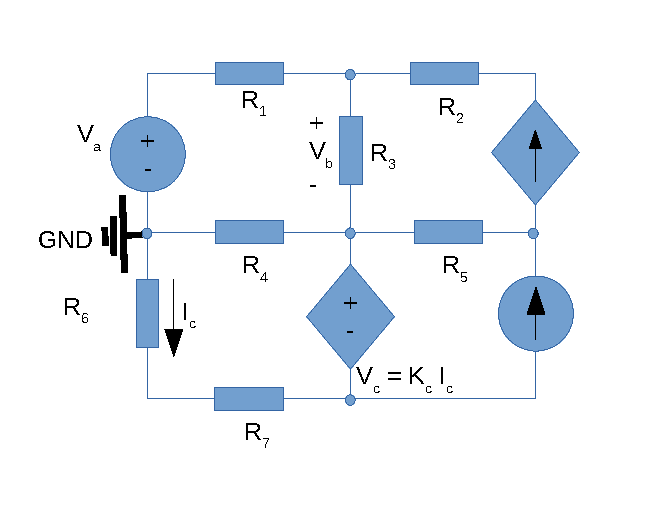
\includegraphics[width=0.7\linewidth]{circ.pdf}
	\caption{Assigned Circuit.}
	\label{fig:circuit}
\end{figure}


